\begin{quote} \textit{7) Se requiere que el regulador actúe en forma automática ante cambios en la carga y/o en la fuente de entrada, para lo cual es necesario diseñar un circuito controlador que sense la tensión de salida y varíe apropiadamente el ciclo de servicio D (reemplazando el generador de pulsos mostrado en el esquema presentado en esta actividad). Esto puede lograrse con un circuito auotoscilante (generalmente discreto con unos pocos transistores) o con un circuito integrado dedicado. Investigar ambas soluciones y plantear una adecuada.}
\end{quote}


Con el fin de realizar un análisis cualitativo del circuito autosclilante en régimen permanente, se representa a la tensión entregada por el rectificador con un tensión constante $Vi$, según se indica en la Figura \ref{fig:cto_auto}. 

\begin{figure}[H]
	\centering
	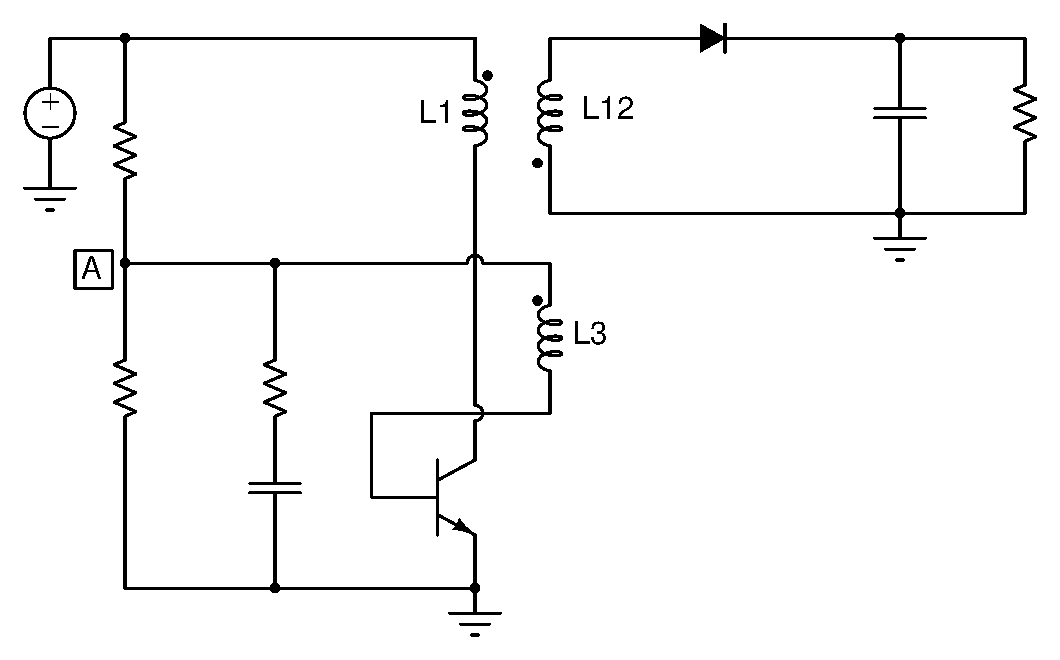
\includegraphics[scale=0.4]{Figuras/auto.eps}
	\caption{Circuito autosclilante.}
	\label{fig:cto_auto}
\end{figure}


En principio en el nodo A, hay una tensión positiva, por lo que el transistor esta en conducción, por lo que circula una corriente IL. Por inducción hay una corriente de salida ya que el diodo D1 está en directa. A su vez se genera una tensión inducida en L3, inversa a la de entrada, por ende el transistor entrará en corte. \\


El controlador puede implementarse mediante el circuito integrado \texttt{TL494}, según se indica en la Figura \ref{fig:cto_tl494}. El controlador actúa como un realimentador, toma una muestra de la tensión de salida y la compara con una tensión de referencia mediante un amplificador de error. Ante una variació en la salida, cambia la tensión en el \textit{gate} del MOSFET y por ende la corriente que circula por el inductor primario. De esta manera se logra regular le ciclo de trabajo D.


\begin{figure}[H]
	\centering
	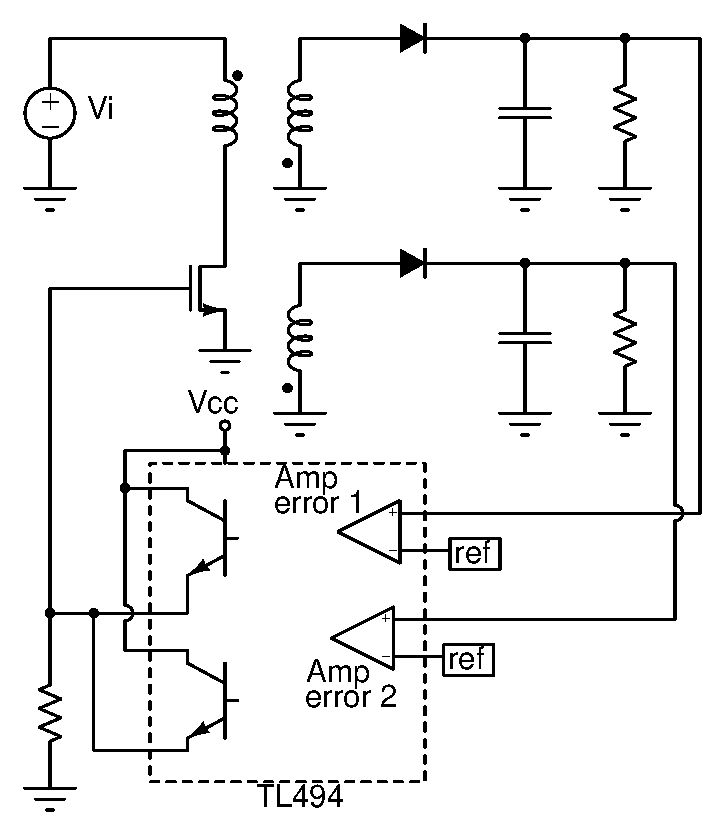
\includegraphics[scale=0.4]{Figuras/tl494.eps}
	\caption{Controlador con \texttt{TL494}.}
	\label{fig:cto_tl494}
\end{figure}

